\documentclass[tikz,border=2pt]{standalone}
\usepackage[T1]{fontenc}
\usepackage{helvet}
\usepackage{amssymb}
\renewcommand{\familydefault}{\sfdefault}
\usetikzlibrary{arrows.meta,calc,positioning}

\definecolor{PanelBlue}{HTML}{2A7DE1}
\definecolor{PanelOrange}{HTML}{FF7A27}
\definecolor{PanelRed}{HTML}{E31A1C}
\definecolor{TextBlack}{HTML}{242424}
\definecolor{Muted}{HTML}{66707C}
\definecolor{BlueFill}{HTML}{F4F8FF}
\definecolor{OrangeFill}{HTML}{FFF8F2}
\definecolor{RedFill}{HTML}{FFF7F7}
\definecolor{LightBlue}{HTML}{C8DEF8}
\definecolor{LightOrange}{HTML}{FFD4B8}
\definecolor{LightRed}{HTML}{FFC6C6}
\definecolor{BarA}{HTML}{4FA0C8}
\definecolor{BarB}{HTML}{8572E8}
\definecolor{BarC}{HTML}{DF762D}
\definecolor{GreyBar}{HTML}{E9E9E9}

\tikzset{
  panel/.style={rounded corners=7pt, line width=0.95pt, fill=white},
  badge/.style={circle, inner sep=0pt, minimum size=0.44cm, font=\bfseries\small, text=white},
  paneltitle/.style={font=\bfseries\large, text=TextBlack, anchor=west},
  panelsub/.style={font=\scriptsize, text=Muted, anchor=west},
  source/.style={rounded corners=5pt, line width=0.55pt, draw=LightBlue, fill=BlueFill,
    text width=1.68cm, minimum height=0.82cm, align=center, inner sep=3pt},
  sourceTitle/.style={font=\bfseries\fontsize{5.8}{6.4}\selectfont, text=TextBlack},
  sourceNote/.style={font=\fontsize{4.7}{5.2}\selectfont, text=Muted},
  card/.style={rounded corners=5pt, line width=0.55pt, align=center, inner sep=4pt},
  inputCard/.style={card, draw=LightOrange, fill=OrangeFill, text width=2.15cm, minimum height=0.95cm},
  outputCard/.style={card, draw=LightRed, fill=RedFill, text width=2.55cm, minimum height=0.72cm},
  trajCard/.style={card, draw=LightOrange, fill=white, text width=1.65cm, minimum height=1.12cm},
  metricCard/.style={card, draw=LightRed, fill=white, text width=3.95cm, minimum height=0.54cm},
  head/.style={font=\bfseries\scriptsize, text=TextBlack, align=center},
  sub/.style={font=\fontsize{5.2}{5.9}\selectfont, text=Muted, align=center},
  micro/.style={font=\fontsize{4.7}{5.2}\selectfont, text=Muted, align=center},
  flow/.style={-{Latex[length=2.2mm,width=1.8mm]}, line width=0.75pt},
  softflow/.style={-{Latex[length=1.8mm,width=1.4mm]}, line width=0.55pt},
}

\newcommand{\SourceTitle}[1]{{\bfseries\fontsize{5.8}{6.4}\selectfont\color{TextBlack}#1}}
\newcommand{\SourceNote}[1]{{\fontsize{4.7}{5.2}\selectfont\color{Muted}#1}}
\newcommand{\Head}[1]{{\bfseries\scriptsize\color{TextBlack}#1}}
\newcommand{\Sub}[1]{{\fontsize{5.2}{5.9}\selectfont\color{Muted}#1}}
\newcommand{\Micro}[1]{{\fontsize{4.7}{5.2}\selectfont\color{Muted}#1}}

\newcommand{\miniDoc}[3]{%
  \begin{scope}[shift={(#1,#2)}, scale=#3]
    \draw[PanelBlue, line width=0.42pt, fill=white] (0.00,0.00) rectangle (0.42,0.52);
    \draw[PanelBlue, line width=0.42pt, fill=white] (0.08,0.08) rectangle (0.50,0.60);
    \draw[PanelBlue, line width=0.34pt] (0.17,0.44) -- (0.40,0.44);
    \draw[PanelBlue, line width=0.34pt] (0.17,0.32) -- (0.40,0.32);
    \draw[PanelBlue, line width=0.34pt] (0.17,0.20) -- (0.40,0.20);
  \end{scope}
}

\newcommand{\profileIcon}[3]{%
  \begin{scope}[shift={(#1,#2)}, scale=#3]
    \draw[PanelBlue, line width=0.45pt, fill=white] (0,0) rectangle (0.55,0.42);
    \draw[PanelBlue!45, line width=0.42pt] (0.12,0.22) -- (0.43,0.22);
  \end{scope}
}

\newcommand{\trajectoryBars}[3]{%
  \begin{scope}[shift={(#1,#2)}]
    #3
  \end{scope}
}

\begin{document}
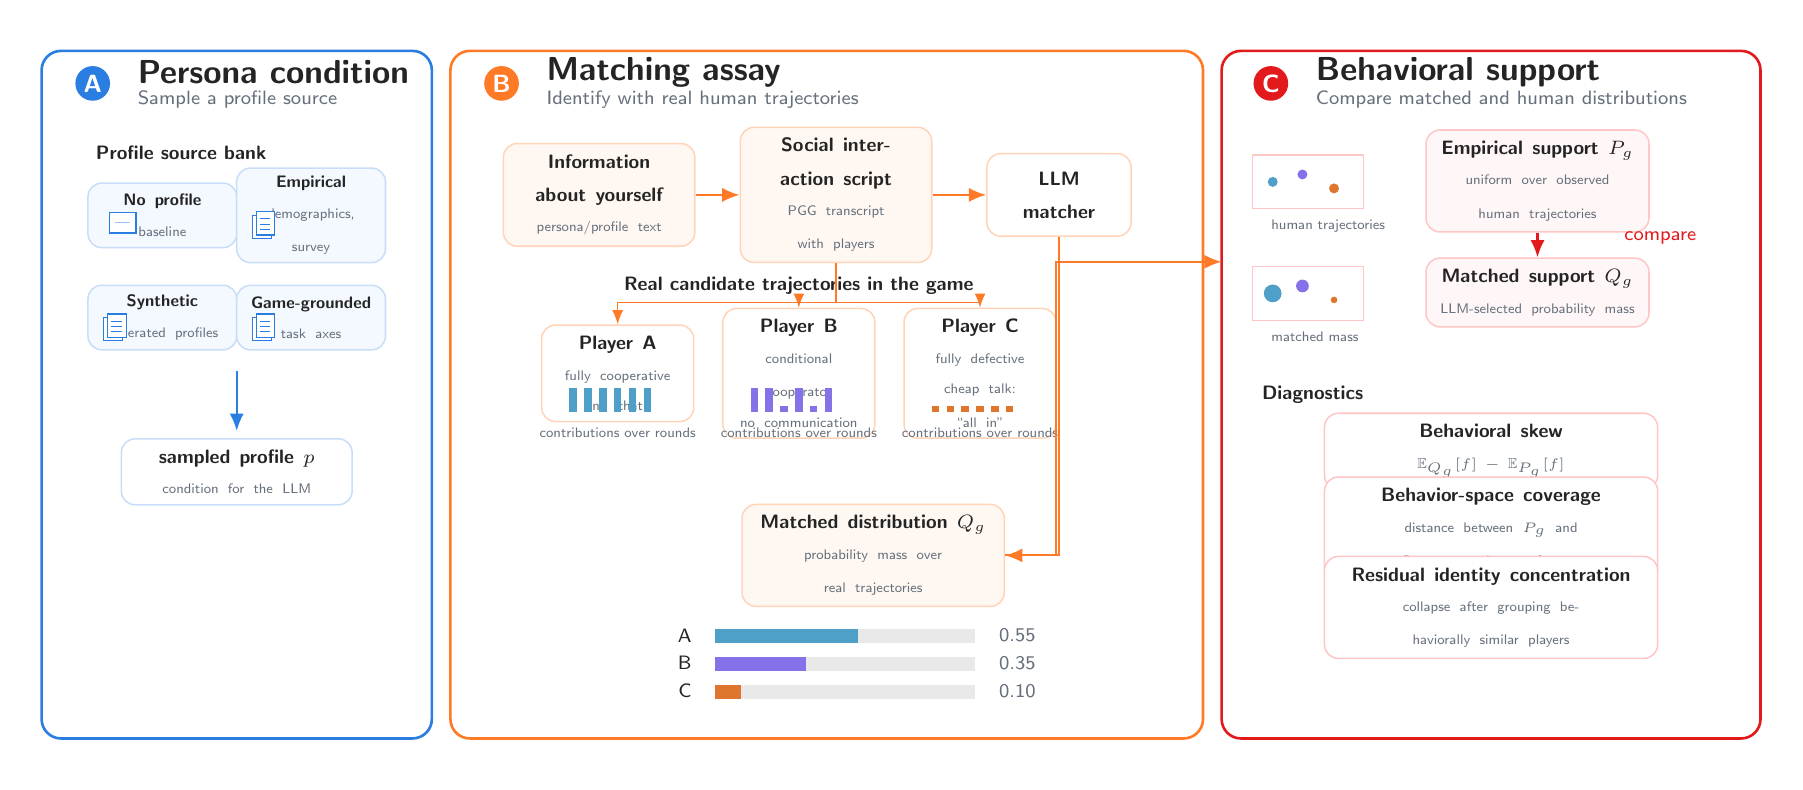
\begin{tikzpicture}[x=1.18cm,y=1.18cm]
  \path[use as bounding box] (0,0) rectangle (18.8,7.9);

  % Panel frames.
  \draw[panel, draw=PanelBlue] (0.15,0.25) rectangle (4.35,7.65);
  \draw[panel, draw=PanelOrange] (4.55,0.25) rectangle (12.65,7.65);
  \draw[panel, draw=PanelRed] (12.85,0.25) rectangle (18.65,7.65);

  % Headers.
  \node[badge, fill=PanelBlue] at (0.70,7.30) {A};
  \node[paneltitle] at (1.08,7.42) {Persona condition};
  \node[panelsub] at (1.08,7.12) {Sample a profile source};

  \node[badge, fill=PanelOrange] at (5.10,7.30) {B};
  \node[paneltitle] at (5.48,7.42) {Matching assay};
  \node[panelsub] at (5.48,7.12) {Identify with real human trajectories};

  \node[badge, fill=PanelRed] at (13.38,7.30) {C};
  \node[paneltitle] at (13.76,7.42) {Behavioral support};
  \node[panelsub] at (13.76,7.12) {Compare matched and human distributions};

  % Panel A: compact source bank.
  \node[font=\bfseries\scriptsize, text=TextBlack, anchor=west] at (0.63,6.55) {Profile source bank};

  \node[source] (noprof) at (1.45,5.88) {\SourceTitle{No profile}\\[-1pt]\SourceNote{baseline}};
  \node[source] (empirical) at (3.05,5.88) {\SourceTitle{Empirical}\\[-1pt]\SourceNote{demographics, survey}};
  \node[source] (synthetic) at (1.45,4.78) {\SourceTitle{Synthetic}\\[-1pt]\SourceNote{generated profiles}};
  \node[source] (grounded) at (3.05,4.78) {\SourceTitle{Game-grounded}\\[-1pt]\SourceNote{task axes}};

  \profileIcon{0.88}{5.69}{0.52}
  \miniDoc{2.42}{5.63}{0.48}
  \miniDoc{0.82}{4.53}{0.48}
  \miniDoc{2.42}{4.53}{0.48}

  \draw[flow, PanelBlue] (2.25,4.20) -- (2.25,3.56);
  \node[card, draw=LightBlue, fill=white, text width=2.65cm, minimum height=0.64cm] (sampled) at (2.25,3.12)
    {\Head{sampled profile $p$}\\[-1pt]\Sub{condition for the LLM}};

  % Panel B: matching assay.
  \node[inputCard] (profile) at (6.15,6.10)
    {\Head{Information about yourself}\\[-1pt]\Sub{persona/profile text}};
  \node[inputCard] (script) at (8.70,6.10)
    {\Head{Social interaction script}\\[-1pt]\Sub{PGG transcript with players}};

  \draw[flow, PanelOrange] (profile.east) -- (script.west);

  \node[card, draw=LightOrange, fill=white, text width=1.55cm, minimum height=1.05cm] (llm) at (11.10,6.10)
    {\Head{LLM}\\\Head{matcher}};
  \draw[flow, PanelOrange] (script.east) -- (llm.west);

  \node[font=\bfseries\scriptsize, text=TextBlack] at (8.30,5.12) {Real candidate trajectories in the game};

  \node[trajCard] (pa) at (6.35,4.18)
    {\Head{Player A}\\[-1pt]\Sub{fully cooperative}\\[-1pt]\Micro{no chat}};
  \node[trajCard] (pb) at (8.30,4.18)
    {\Head{Player B}\\[-1pt]\Sub{conditional cooperator}\\[-1pt]\Micro{no communication}};
  \node[trajCard] (pc) at (10.25,4.18)
    {\Head{Player C}\\[-1pt]\Sub{fully defective}\\[-1pt]\Micro{cheap talk: ``all in''}};

  % Behavior miniatures.
  \foreach \i in {0,...,5}{\fill[BarA] (5.83+\i*0.16,3.76) rectangle +(0.08,0.26);}
  \foreach \i/\h in {0/0.26,1/0.26,2/0.07,3/0.26,4/0.07,5/0.26}{\fill[BarB] (7.78+\i*0.16,3.76) rectangle +(0.08,\h);}
  \foreach \i in {0,...,5}{\fill[BarC] (9.73+\i*0.16,3.76) rectangle +(0.08,0.07);}

  \node[micro] at (6.35,3.54) {contributions over rounds};
  \node[micro] at (8.30,3.54) {contributions over rounds};
  \node[micro] at (10.25,3.54) {contributions over rounds};

  \draw[softflow, PanelOrange] (script.south) -- ++(0,-0.42) -| (pa.north);
  \draw[softflow, PanelOrange] (script.south) -- ++(0,-0.42) -| (pb.north);
  \draw[softflow, PanelOrange] (script.south) -- ++(0,-0.42) -| (pc.north);

  \node[card, draw=LightOrange, fill=OrangeFill, text width=3.05cm, minimum height=0.86cm] (qbox) at (9.10,2.22)
    {\Head{Matched distribution $Q_g$}\\[-1pt]\Sub{probability mass over real trajectories}};

  \draw[flow, PanelOrange] (llm.south) |- (qbox.east);
  \node[font=\scriptsize, text=TextBlack, anchor=east] at (7.25,1.36) {A};
  \fill[GreyBar] (7.40,1.28) rectangle (10.20,1.43);
  \fill[BarA] (7.40,1.28) rectangle (8.94,1.43);
  \node[font=\scriptsize, text=Muted, anchor=west] at (10.35,1.36) {0.55};

  \node[font=\scriptsize, text=TextBlack, anchor=east] at (7.25,1.06) {B};
  \fill[GreyBar] (7.40,0.98) rectangle (10.20,1.13);
  \fill[BarB] (7.40,0.98) rectangle (8.38,1.13);
  \node[font=\scriptsize, text=Muted, anchor=west] at (10.35,1.06) {0.35};

  \node[font=\scriptsize, text=TextBlack, anchor=east] at (7.25,0.76) {C};
  \fill[GreyBar] (7.40,0.68) rectangle (10.20,0.83);
  \fill[BarC] (7.40,0.68) rectangle (7.68,0.83);
  \node[font=\scriptsize, text=Muted, anchor=west] at (10.35,0.76) {0.10};

  \draw[flow, PanelOrange] (qbox.east) -- ++(0.55,0) |- (12.85,5.38);

  % Panel C: P_g vs Q_g comparison.
  \node[outputCard] (pg) at (16.25,6.25)
    {\Head{Empirical support $P_g$}\\[-1pt]\Sub{uniform over observed human trajectories}};
  \node[outputCard] (qg) at (16.25,5.05)
    {\Head{Matched support $Q_g$}\\[-1pt]\Sub{LLM-selected probability mass}};

  \draw[flow, PanelRed] (pg.south) -- (qg.north);
  \node[font=\scriptsize, text=PanelRed, anchor=west] at (17.08,5.64) {compare};

  % Schematic behavior-space dots.
  \begin{scope}[shift={(13.18,5.95)}]
    \draw[LightRed, line width=0.42pt] (0,0) rectangle (1.20,0.58);
    \fill[BarA] (0.22,0.29) circle (1.8pt);
    \fill[BarB] (0.54,0.37) circle (1.8pt);
    \fill[BarC] (0.88,0.22) circle (1.8pt);
    \node[micro, anchor=west] at (0.10,-0.18) {human trajectories};
  \end{scope}
  \begin{scope}[shift={(13.18,4.75)}]
    \draw[LightRed, line width=0.42pt] (0,0) rectangle (1.20,0.58);
    \fill[BarA] (0.22,0.29) circle (3.2pt);
    \fill[BarB] (0.54,0.37) circle (2.3pt);
    \fill[BarC] (0.88,0.22) circle (1.2pt);
    \node[micro, anchor=west] at (0.10,-0.18) {matched mass};
  \end{scope}

  \node[font=\bfseries\scriptsize, text=TextBlack, anchor=west] at (13.18,3.95) {Diagnostics};

  \node[metricCard] at (15.75,3.34)
    {\Head{Behavioral skew}\\[-1pt]\Sub{$\mathbb{E}_{Q_g}[f]-\mathbb{E}_{P_g}[f]$}};
  \node[metricCard] at (15.75,2.50)
    {\Head{Behavior-space coverage}\\[-1pt]\Sub{distance between $P_g$ and $Q_g$ over trajectory features}};
  \node[metricCard] at (15.75,1.66)
    {\Head{Residual identity concentration}\\[-1pt]\Sub{collapse after grouping behaviorally similar players}};
\end{tikzpicture}
\end{document}
